\chapter{Daemon d'interface avec le GPS}

Sur Linux, il ne convient généralement pas de gérer les périphériques utilisant l'UART avec des drivers. En effet à la différence des bus de communications comme I2C ou SPI, l'UART dispose déjà d'un driver permettant d'envoyer et de recevoir des trames depuis l'espace utilisateur. Les drivers résidant eux dans l'espace du système d'exploitation.

De plus l'UART est d'un niveau d'abstraction supérieur par rapport à ces bus puisqu'il ne s'agit pas d'envoyer des commandes de lecture ou d'écriture sur les registres du périphérique mais d'envoyer des trames de commande que le périphérique va interpréter.

\vspace{1cm}

On utilise donc généralement des daemons pour faire l'interface avec ce type de périphériques. Les daemons étant des programmes tournant en tâche de fond de l'espace utilisateur du système.

%fonctionnement gps, trames NMEA
%configuration gps
\section{Fonctionnement du GPS}

Le GPS utilise des trames NMEA, qui est une norme de communication américaine pour les équipements marins. Elle est largement utilisée par les GPS.

\vspace{1cm}

Il existe de nombreuses trames NMEA, toutes sont préfixées de \codeinline{text}{$} et suffixées de \mintinline[fontsize=\footnotesize]{text}{\r\n}. Les deux premiers caractères après \codeinline{text}{$} désignent le type d'équipement qui émet la trame, une trame émise par un GPS commence par \codeinline{text}{GP}. Elles comportent également un CRC, calculé par XOR des codes ASCII des précédents caractères.

Ce GPS dispose également d'un jeu de trames propre au constructeur, composé de commandes et de réponses, commençant par \codeinline{text}{PMTK}.

\vspace{1cm}

Le GPS envoie périodiquement certaines trames NMEA et répond aux instructions que l'on peut lui envoyer.

Parmi les trames intéressantes qu'envoie le GPS, on trouve~:
\begin{itemize}[label=$\bullet$]
	\item \codeinline{text}{GPGLL}~: Contient notamment la latitude et la longitude.
	\item \codeinline{text}{GPRMC}~: Contient notamment la latitude et la longitude.
	\item \codeinline{text}{GPGGA}~: Contient notamment la latitude, la longitude et l'altitude.
	\item \codeinline{text}{PMTK705}~: Contient le nom et la version du firmware du GPS. Réponse à la trame de requête \codeinline{text}{PMTK605}.
	\end{itemize}

\vspace{1cm}

La trame \codeinline{text}{GPGGA} est celle qui contient le plus d'informations intéressantes. À titre d'exemple, voici sa décomposition~:

\mintinline[fontsize=\footnotesize]{text}{$GPGGA,204444.000,4042.6250,N,07400.5054,W,1,6,1.45,278.7,M,-34.2,M,,*6C\r\n}

\begin{itemize}[label=$\bullet$]
		\item \codeinline{text}{204444.000}~: Heure de calcul de la position $20h44m44s$
		\item \codeinline{text}{4042.6250,N}~: Latitude $40$°$42'62,50"$ Nord
		\item \codeinline{text}{07400.5054,W}~: Longitude $074$°$00'50,54"$ Est
		\item \codeinline{text}{1}~: Indicateur de qualité 1 = GPS
		\item \codeinline{text}{6}~: Nombre de satellites utilisés
		\item \codeinline{text}{1.45}~: Dilution de la position horizontale (HDOP)
		\item \codeinline{text}{278.7,M}~: Altitude par rapport au niveau moyen de la mer $278,7m$
		\item \codeinline{text}{-34.2,M}~: Hauteur du géoïde $-34,2m$
		\item \codeinline{text}{vide}~: Age des données GPS différentiel
		\item \codeinline{text}{vide}~: Identifient de la station GPS différentiel
		\item \codeinline{text}{6C}~: CRC de \codeinline{text}{GPGGA,204444.000,4042.6250,N,07400.5054,W,1,6,1.45,278.7,M,-34.2,M,,*}
		\end{itemize}

\vspace{1cm}

La trame \codeinline{text}{GPGGA} contenant toutes les informations utiles, il semble inutile de laisser le GPS envoyer périodiquement d'autres trames que celle-ci.

La trame de commande \codeinline{text}{314 PMTK_API_SET_NMEA_OUTPUT} permet de configurer les trames qu'envoie périodiquement le GPS~:

\mintinline[fontsize=\footnotesize]{text}{$PMTK314,0,0,0,1,0,0,0,0,0,0,0,0,0,0,0,0,0,0,0*29\r\n}

\begin{itemize}[label=$\bullet$]
	\item \codeinline{text}{GPGLL}~: Trame jamais envoyée.
	\item \codeinline{text}{GPRMC}~: Trame jamais envoyée.
	\item \codeinline{text}{GPVTG}~: Trame jamais envoyée.
	\item \codeinline{text}{GPGGA}~: Trame envoyée une fois tous les \codeinline{text}{1} calcul de position. Peut aller jusqu'à une trame tous les \codeinline{text}{5} calculs de position.
	\item \codeinline{text}{GPGSA}~: Trame jamais envoyée.
	\item \codeinline{text}{GPGSV}~: Trame jamais envoyée.
	\item Les autres champs doivent rester à \codeinline{text}{0}.
	\item \codeinline{text}{29}~: CRC de \codeinline{text}{PMTK314,0,0,0,1,0,0,0,0,0,0,0,0,0,0,0,0,0,0,0*}
	\end{itemize}

\vspace{1cm}

Le GPS doit alors répondre une trame \codeinline{text}{001 PMTK_ACK}~: \mintinline[fontsize=\footnotesize]{text}{$PMTK001,314,3*36\r\n} signifiant que la commande a été prise en compte.

\section{Fonctionnement du daemon}

\begin{figure}[H]
    \centering
    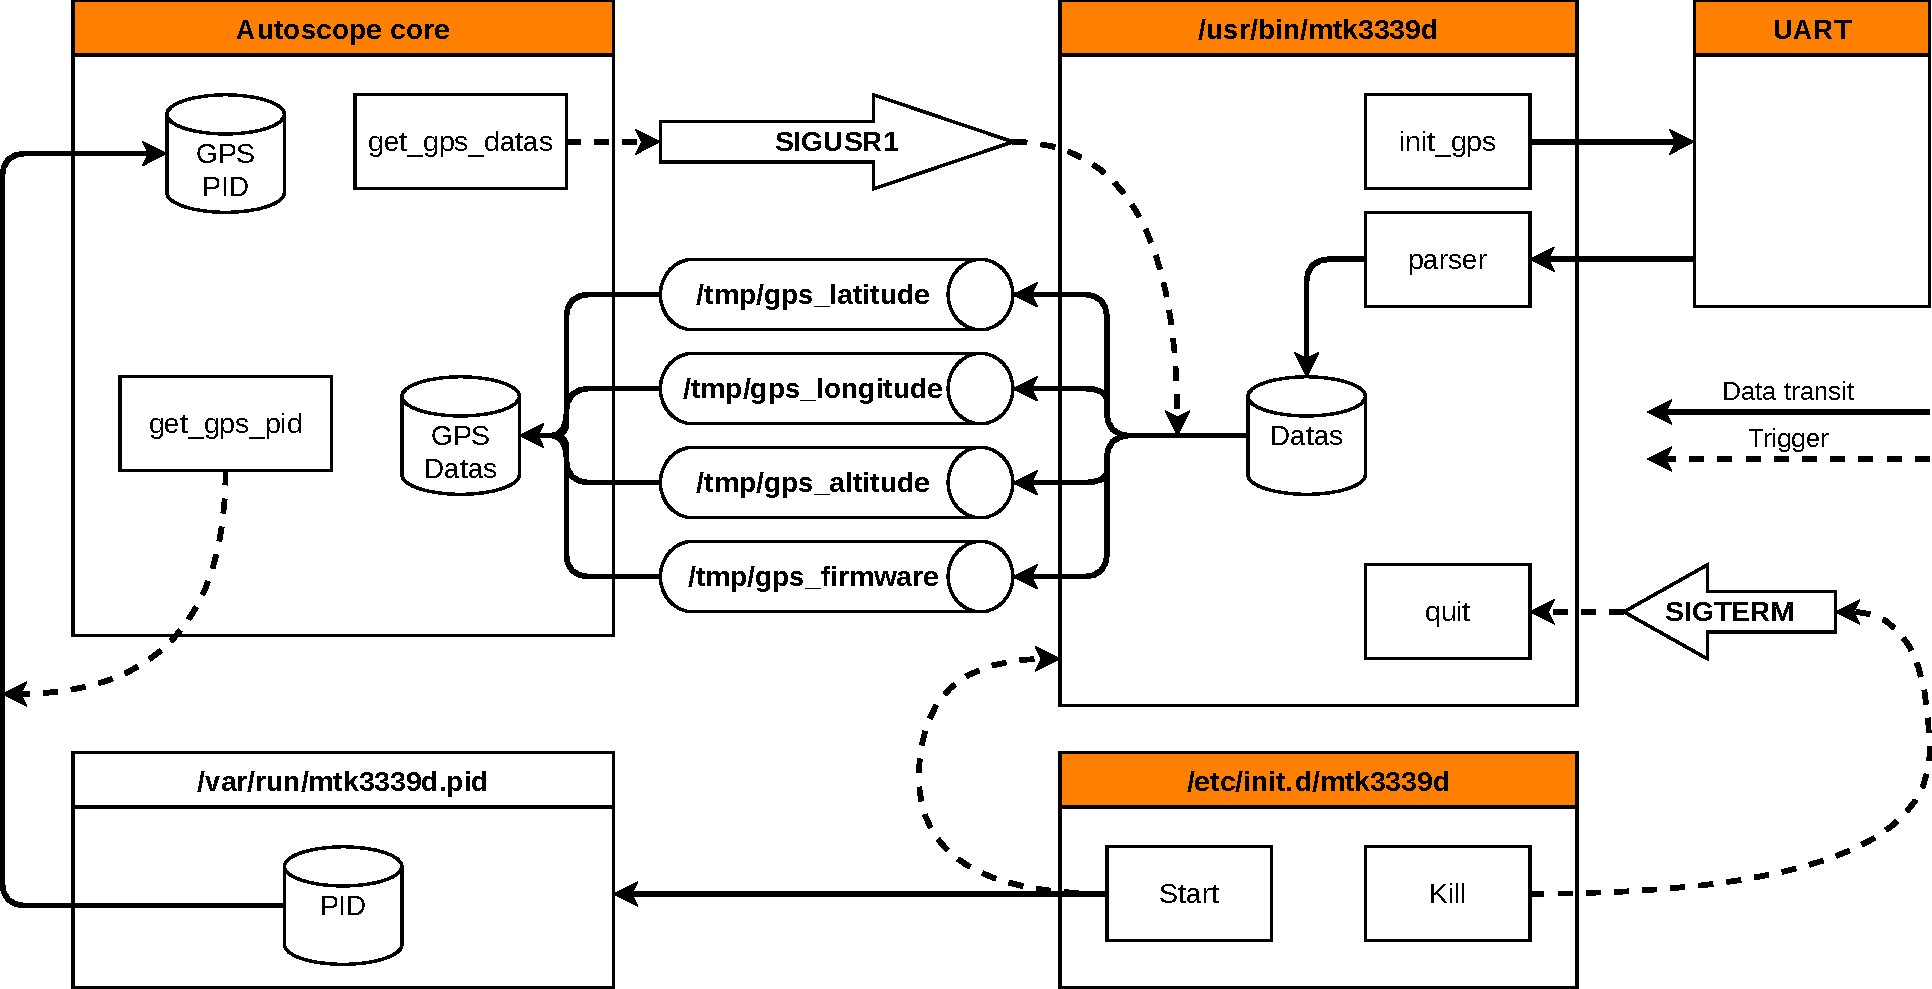
\includegraphics[width=1\linewidth]{sch_mtk3339d.pdf}
    \decoRule
    \caption[
    Architecture logicielle du daemon d'interface avec le GPS]{
    Architecture logicielle du daemon d'interface avec le GPS}
    \label{fig:Architecture logicielle du daemon d'interface avec le GPS}
	\end{figure}

\vspace{1cm}

Le daemon \codeinline{text}{/usr/bin/mtk3339d} est invoqué et tué par son script d'initialisation\\\codeinline{text}{/etc/init.d/mtk3339d}.

\vspace{1cm}

Lors de son fonctionnement, il réceptionne les trames envoyées par le GPS sur la liaison série et en extrait les données intéressantes qu'il stocke dans sa mémoire. Ces données sont la latitude, la longitude, l'altitude, ainsi que le nom et la version du firmware, utilisés principalement comme débug.

La communication de ces données au logiciel principal du télescope se fait à la demande de ce dernier et par le biais d'un pipe FIFO pour chaque donnée.

\vspace{1cm}

Pour adresser sa requête des données au daemon (matérialisée par l'envoi d'un signal \codeinline{text}{SIGUSR1}), le logiciel principal a besoin de connaître le \codeinline{text}{PID} du daemon. Celui-ci est stocké dans le fichier \codeinline{text}{/var/run/mtk3339d.pid} créé par le script d'initialisation lors de l'invocation du daemon.

\vspace{1cm}

La fonction \codeinline{text}{init_gps} envoie la trame de configuration \codeinline{text}{PMTK314} décrite précédemment ainsi qu'une trame de requête des informations firmware \codeinline{text}{PMTK605}.

%\vspace{1cm}
\newpage

À l'usage, le daemon se lance automatiquement à l'allumage du système. On peut alors utiliser un programme de test \codeinline{text}{mtk3339d-test} contenant le fragment décrit ci-dessus du programme principal du télescope. Le test n'a pas eu l'occasion d'être fait dans un environnement où le GPS parvient à se connecter aux satellites, d'où les données nulles~:

\code{text}
root@autoscope ~ #
    mtk3339d-test
        GPS daemon PID : 335
        Recieved latitude : 0
        Recieved longitude : 0
        Recieved altitude : 0
        Recieved firmware : AXN_2.31_3339_13101700
\end{minted}

